\documentclass[11pt]{article}

\usepackage[utf8]{inputenc}
\usepackage[T1]{fontenc}
\usepackage[english, french]{babel} %français
\usepackage{amsmath}
\usepackage{amsfonts}
\usepackage{makeidx}
\usepackage{graphicx}
\usepackage[left=2cm,right=2cm,top=2cm,bottom=2cm]{geometry}
\usepackage{mathtools} %dcases
\usepackage{braket} %quantum mechanics
\usepackage[colorlinks=true, linkcolor=black, citecolor=black]{hyperref} % hyperlinks
\usepackage{tikz} % drawing in LaTeX
\usepackage{ dsfont } % hollow letters

% compile child documents using this preamble
\usepackage{subfiles}

% compile child files with separate preambles, and include them in the document
\usepackage{standalone}

% subfigure
\usepackage{caption}
\usepackage{subcaption}

% the equal sign I use to define something
\newcommand{\define}{\ensuremath{ \overset{\text{def}}{=} }}

% differential element
\renewcommand{\d}[1]{\mathrm{d}#1}

% similar symbol with a limit underneath
\newcommand{\simlim}[2]{\ensuremath{ \underset{#1 \rightarrow #2}{\sim} }}

\newcommand{\om}{\ensuremath{\omega}}
\newcommand{\lb}{\ensuremath{\overline{\lambda}}}
\newcommand{\zb}{\ensuremath{\overline{z}}}

\title{\textbf{Fractal dimensions of quasicrystalline chains \emph{via} a perturbative renormalization group.}}
\author{}
\date{}
\begin{document}

\selectlanguage{english}

\maketitle

%\abstract{}

We focus on tight-binding Hamiltonians on one-dimensional quasiperiodic tilings.
Notable examples include the Harper model, and the family of quasiperiodic Hamiltonians constructed by the cut and project method. 
Each of the latter is associated with an irrational number, $\alpha$.
It has the geometrical interpretation of the tangent of the angle between the projection axis and the direction of one of the basis vectors of the two-dimensional superlattice.
The Hamiltonian of such a model writes
\begin{equation}
	H^\alpha = \sum_i t^\alpha_i \left( \ket{i} \bra{i+1} + \ket{i+1} \bra{i} \right)
\end{equation}
where the jump amplitudes $t^\alpha_i$ can take two values $t_s$, $t_w$:
\begin{equation}
	t_i^\alpha = \begin{dcases*}
	t_w & when $i \bmod(1+\alpha) \geq \alpha$, \\
	t_s & otherwise.
	\end{dcases*}
\end{equation}
If we replace the irrational $\alpha$ by a rational approximation $\alpha_n = p_n/q_n$, the sequence of couplings is modified:
\begin{equation}
	t_i^{p_n/q_n} = \begin{dcases*}
	t_w & when $q_n i \bmod(p_n+q_n) \geq p_n$, \\
	t_s & otherwise,
	\end{dcases*}
\end{equation}
and we obtain a periodic system of period $p_n + q_n$. 
Thus, to a sequence of rationals $\{\alpha_n\}_n$ converging to $\alpha$ is associated in a natural way a sequence of periodic tight-binding Hamiltonians -- called approximants, converging to a quasiperidic Hamiltonian. We will call $H_n$ the $n^\text{th}$ approximant, generated by the rationnal $\alpha_n$.


Amongst all irrationals, the golden ratio and its inverse, $\omega = 2/(1+\sqrt{5})$, play a special role. They contain only the number 1 in their continued fraction expansion. In that sense, these two numbers are the hardest to approximate by rationnals. 
We thus expect the quasiperiodicity to have the most spectacular consequences when the irrational is taken to be the golden ratio or its inverse.

We restrict ourselves to the case $\alpha \leq 1$ (the other case being equivalent up the exchange of $t_s$ and $t_w$). As an example, we are going to chose $\alpha = \omega$. The tight-binding Hamiltonian resulting from this choice is called the Fibonacci Hamiltonian.
However, our results are general and apply to every Hamiltonian constructed by the cut and project method.

\section{Co-numbering, atoms and molecules.}

We consider a periodic approximant given by the rational $\alpha_n = p_n/q_n$. Later, we are going to specialize to the case of the Fibonacci Hamiltonian, but for the moment we wish to stay as general as possible.
We have already seen already that the integer
\begin{equation}
	i'_k = q_n k \bmod(p_n+q_n)
\end{equation}
determines the sequence of jump amplitudes. How does $i'_k$ changes when we jump from one site to the next, i.e. when we increase $k$ by one unit? It is easy to check that
\begin{equation}
	i'_{k+1} = \begin{dcases*}
	i'_k - p_n & when sites $k$ and $k+1$ are linked by $t_w$, \\
	i'_k + q_n & when sites $k$ and $k+1$ are linked by $t_s$.
	\end{dcases*}
\end{equation}
Thus, the sequence of $i'_k$ furnishes a natural renumbering of the sites, as was first noted by R. Mosseri \cite{Moss}. A generalization of this renumbering to higher dimensional quasicrystals can be found in \cite{MossSire}.
In the basis where sites are numbered using $i'$, up to a suitable shift of the origin, the Hamiltonian rewrites as a two-banded Toeplitz matrix:
\begin{equation}
	H_n = 
	\bordermatrix{ 
	 	& 1 	&	\ldots & & p_n	& &  \ldots &	& q_n &	& \ldots	&  \cr
    1 	& 0 		& \ldots & 0 & t_w & 0	& \ldots & 0 & t_s	& 0 		& \ldots		 \cr
    \vdots & & & & & \ddots	& & & & \ddots & \cr
    p_n & t_w \cr
    \vdots & & \ddots \cr
    q_n & t_s \cr
    \vdots & & \ddots \cr
     & 
    }
\end{equation}
The co-numbering allows to distinguish two classes of sites. We call \emph{molecular} the first $p_n$ and the last $p_n$ sites. We call \emph{atomic} the remaining $q_n - p_n$ sites.
Each molecular site is coupled to another molecular site by a $t_s$ coupling, and to an atomic site by a $t_w$ coupling. Thus, in the limit $t_w \ll t_s$, molecular sites form isolated diamtomic \emph{molecules}. 
On the other hand, the atomic sites are all coupled to two molecular sites by $t_w$ couplings. Thus, in the limit $t_w \ll t_s$, they form isolated \emph{atoms}.

Now, we focus on the particular case of the Fibonacci Hamiltonian. 
We take $p_n = F_{n-2}$, $q_n = F_{n-1}$ where $F_n$ is the $n^\text{th}$ Fibonacci number. Then, $\alpha_n = F_{n-2}/F_{n-1}$ indeed approximates the inverse golden ratio, so that we have constructed an approximant to the Fibonacci chain.
The $n^\text{th}$ Fibonacci approximant consists of a block of $F_{n-2} + F_{n-1} = F_{n}$ sites, repeated periodically. That block contain $F_{n-1} - F_{n-2} = F_{n-3}$ atoms and $F_{n-2}$ molecules (that is, $2F_{n-2}$ molecular sites).

Figure \eqref{fig:fib8} shows the molecules and atoms of the fifth Fibonacci approximant, together with the co-numbering of the sites.

\begin{figure}[htp]
	\centering
	\subfile{img/fibonacci_approximant.tex}
	\caption{The periodically repeated block of the fifth approximant to the Fibonacci chain. Weak couplings $t_w$ are represented by a single line, and strong couplings $t_s$ by a double line. Below each site is its co-numbered label.}
\label{fig:fib8}
\end{figure}

\section{Deflation and renormalization}

\subsection{Deflation, molecular and atomic chains.}
Besides the cut and project method, we can construct the Fibonacci chain by inflation.
We start from the trivial chain:
\begin{equation}
	C_0 = t_s
\end{equation}
and we apply repetively the \emph{inflation rule}
\begin{equation}
	r \define \begin{cases}
        t_{w} & \rightarrow t_w t_s \\
        t_s & \rightarrow t_w
      \end{cases}
\end{equation} 
on it to build new chains: $C_1 = r(C_0) = t_w$, $C_2 = r(C_1) = t_w t_s$, ... $C_n = r^n(C_0)$.
Then, perhaps up to a global circular permutation of the couplings, the infinite chain $C_n C_n C_n \dots$ is the sequence of couplings of the $n^\text{th}$ approximant.
Furthermore, we can define \emph{deflation rules} relating an approximant to a smaller one.
The \emph{molecular deflation rule}
\begin{equation}
	d_m = \begin{cases}
        t_{w} & \leftarrow t_s t_w t_w (t_s)\\
        t_s & \leftarrow t_s t_w (t_s)
      \end{cases}
\end{equation}
decimates all sites except molecular ones. Fig. \eqref{fig:mol_defl} examplifies the decimation operation.
Crucially, the deflated chain is again a Fibonacci chain. More precisely, the molecular deflation relates the approximant of size $n$ to the approximant of size $n-2$: $d_m(C_n C_n \dots) = C_{n-2} C_{n-2} \dots$.

\begin{figure}[htp]
	\centering
	\subfile{img/molecular_deflation.tex}
	\caption{The molecular deflation rule illustrated. Here we relate the fifth approximant to the third.}
\label{fig:mol_defl}
\end{figure}

Similarly, we can perform a decimation operation on all sites except atomic ones. We call such an operation an \emph{atomic decimation}.
Again, the deflated chain is also a Fibonacci chain.
The atomic decimation relates the approximant of size $n$ to the approximant of size $n-3$. 
Fig. \eqref{fig:at_defl} examplifies the procedure.

\begin{figure}[htp]
	\centering
	\subfile{img/atomic_deflation.tex}
	\caption{The atomic deflation rule illustrated. Here we relate the fifth approximant to the second.}
\label{fig:at_defl}
\end{figure}

\subsection{Renormalization}

We are now going to focus on the limit $t_w \ll t_s$, in which the disinction between atomic and molecular sites acquires its real meaning.
We define $\rho = t_w/t_s$. It will be our perturbative parameter.
The energies are at most of order $t_s$. As varying $t_s$ (while keeping $\rho$ fixed) simply amounts to rescaling the whole energy spectrum, we arbitrarily set $t_s = 1$. 

When $\rho = 0$, the atoms and the molecules decouple. The eigenstates are the molecular bonding and antibonding states, at energies $\pm 1$, and the atomic state at zero energy.
The spectrum is constituted of three infinitely degenerated levels.

When $\rho > 0$, $\rho \ll 1$, perturbation theory tells us that states inside each of the three degenerated levels weakly coupled to each other, thus raising the degeneracy.
Let us focus to begin with on atomic states. At first order, each atomic site is coupled to the neighbouring atomic sites.
Effectively, we can therefore work on the \emph{deflated} chain, with effective hopping amplitudes coupling atomic sites. Perturbation theory gives us the expression of the effective hopping amplitudes \cite{Niu1990}.
We find
\begin{equation}
	\begin{dcases}
	t^\text{atomic}_w &= \zb \rho\\
	t^\text{atomic}_s &= \zb,
	\end{dcases}
\end{equation}
with $\zb =\rho^2$.

Similarly, each molecular site is coupled to the neighbouring molecular sites. 
There is here a small subtlety. A molecule sits on two neighbouring sites. Say for example that that sites $i$ and $i+1$ on the chain form a molecule.
Then, by a change of basis, we can say that the molecule sits at the ``bonding'' and ``antibonding'' \emph{effective} sites respectively given by the linear combination of the localized states $\ket{i} + \ket{i+1}$ and $\ket{i} - \ket{i+1}$.
It is natural to do that, because when $\rho = 0$ the molecular eigenstates are localized in this new basis.
At first order, the bonding sites of neighbouring molecules couple to each other. 
This results in effective hopping amplitudes given by
\begin{equation}
	\begin{dcases}
	t^\text{bonding}_w &= z \rho\\
	t^\text{bonding}_s &= z,
	\end{dcases}
\end{equation}
with $z = \rho/2$. This also results in the appearance of an onsite potential, $V^\text{bonding}  = -1$. 
The antibonding sites similarly couple to each other, resulting in the same effective hopping terms, but in a different onsite potential, $V^\text{antibonding} = +1$.

To summarize, we have seen that we can formally separate the chain of the $n^\text{th}$ approximant into molecular and atomic chains.
In the limit $\rho \ll 1$, the Hamiltonian of the $n^\text{th}$ approximant decouples into the direct sum of three Hamiltonians: an atomic Hamiltonian living on the chain formed of atomic sites, a bonding Hamiltonian living on the chain formed of molecular bonding sites, and an antibonding Hamiltonian living on the chain formed of molecular antibonding sites. 
Because the atomic and molecular chains are again Fibonacci chains (but of smaller lengths), these three Hamiltonians are Fibonacci Hamiltonians, with renormalized hopping terms and onsite energies.
Formally, we have:
\begin{equation}
\label{eq:recur_ham}
	H_n = \underbrace{\left( z H_{n-2} - 1 \right)}_{\text{bonding sites}} \oplus \underbrace{\left( \zb H_{n-3} \right)}_{\text{atomic sites}} \oplus \underbrace{\left( z H_{n-2} + 1 \right)}_{\text{antibonding sites}} + \mathcal{O}(\rho^4)
\end{equation}

In the limit $n \rightarrow \infty$, the chain becomes quasiperiodic. As such, we expect its wavefunctions and its spectrum to be nontrivial, namely to exhibit multifractality.
We are going to try using the recursion relation we have on the Hamiltonians of the approximants to derive recursion relations on energies and wavefunctions. In this way, we hope to gain some insight on the form of the spectrum and of the wavefunctions in the limit $n \rightarrow \infty$.
From that, we hope to characterize the multifractality of the quasiperiodic chain by computing the fractal dimensions of its wavefunctions and of its spectrum.

\subsection{Renormalization paths, equivalence between energy labels and co-numbers.}

%The co-numbering naturally distinguishes between molecules and atoms.
%For the $n^\text{th}$ approximant, the first $p_n = F_{n-2}$ sites are the left part of a molecule. We will attach to these sites a label $m_l$. The next $q_n - p_n = F_{n-3}$ sites are the atomic sites, and we will label then $a$. The last $p_n = F_{n-2}$ sites are the right part of a molecule, we will label them $m_r$.
%We can repeat this procedure at the step $n-2$ for molecular sites, $n-3$ for atomic sites, until we reach the trivial state $n=1$ or $n=0$. 
%We see that there is a one-to-one mapping between the co-number of a site, $i$, and the sequence of labels $l_n l_{n-2/n-3} \dots l_s \dots$, where $l_s = m_l, a$ or $m_r$ is the label of the site at step $s$.

%In the perturbative picture, we can thus represent each state as a sequence of labels, which we call its \emph{renormalization path}. 
%We can plot these sequences on a trifurcating tree (fig. \eqref{fig:tree_states})

Since the Hamiltonian of an approximant is the direct sum of three Hamiltonians, the energy spectrum can be expressed as the union of three spectra.
Specifically, the spectrum $\mathcal{S}_n$ of the $n^\text{th}$ approximant is the union of scaled version of the spectra at step $n-2$ and $n-3$:
\begin{equation}
\label{eq:recur_spectrum}
	\mathcal{S}_n = \left( z \mathcal{S}_{n-2} - 1 \right) \bigcup \left( \zb \mathcal{S}_{n-3} \right) \bigcup \left( z \mathcal{S}_{n-2} + 1 \right) 
\end{equation}

So, we can distinguish between three energy clusters: the antibonding molecular energy cluster, the atomic energy cluster and the bonding energy cluster. Molecular clusters are separated from the atomic cluster by a gap of width $\Delta \sim 1 - z$.

Relation \eqref{eq:recur_spectrum} tells us that each of these three clusters is the spectrum of a smaller approximant, and as such, it decomposes in its turn into three bands, etc.
The spectrum has therefore a recursive, Cantor set-like description.

This has an important consequence: we can associate to a given energy level of the $n^\text{th}$ approximant a unique sequence of labels called its \emph{renormalization path} in the following way.
If it is in the upper band, associated to molecular bounding states, we give it a $+$  label.
If it is in the middle band, associated to atomic states, we give it a $0$ label, and if it is in the lower band , associated to molecular antibonding states we give it a $-$ label.
But then, the cluster our energy level belongs to is again the spectrum of some approximant (of size $n-2$ if it is the upper or lower band, of size $n-3$ if it is the middle band). We can thus repeat this labelling procedure recursively, and indeed assign to each energy level of the $n^\text{th}$ approximant a unique sequence of labels, its renormalization path.
We can plot these sequences on a trifurcating tree (fig. \eqref{fig:tree_en}), as was already pointed out \cite{KaluginKitaevLevitov} \cite{Piechon95}.

\begin{figure}[htp]
\centering
    	\includestandalone{img/energy_tree}
\caption{Trifurcating tree of energies. Each dot symbolizes an energy level. To the right of the deepest energy levels is written their renormalization path.}
\label{fig:tree_en}
\end{figure}

We can also associate to a given site of the $n^\text{th}$ approximant a unique renormalization path in the following way.
If it is an antibonding site, we give it a $+$  label.
If it is an atomic site, we give it a $0$ label, and if it is a bonding site we give it a $-$ label.
But then, the family (bonding, antibonding or atomic) our site belongs to forms again a Fibonacci chain (of size $n-2$ for bonding and antibonding sites, of size $n-3$ for atomic sites). 
Thus, as for energy levels, we can repeat this labelling procedure recursively, and indeed assign to each site of the $n^\text{th}$ approximant a unique renormalization path.

Now, we want to characterize completely the eigenstates of the $n^\text{th}$ approximant. 
Given an energy level, we consider the associated eigenstate. 
Equation  \eqref{eq:recur_ham} tells us that at leading order in $\rho$, the eigenstate has nonzero amplitude only on molecular bonding sites, on atomic sites or on antibonding sites if it associated respectively to an energy in the bonding, in the atomic or in the antibonding energy cluster.
In other words, the eigenstate has nonzero amplitude on a site only if the first letter of its renormalization path is the first lettter of the renormalization path of the energy level of the eigenstate.
We can repeat this reasoning recursively, and we conclude that \emph{the eigenstate has a nonzero amplitude only on sites whose renormalization path matches the one of the energy level}.

\begin{figure}[htp]
\centering
\begin{subfigure}{.5\textwidth}
  \centering
  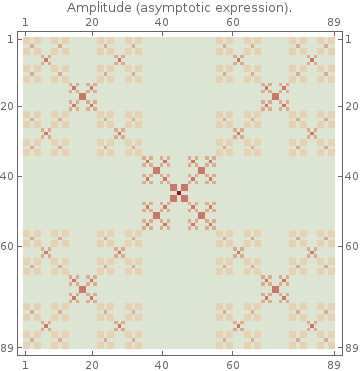
\includegraphics[width=.75\textwidth]{img/amplitude_asym.png}
  \caption{LDoS, asymptoptic expression.}
  \label{fig:wf_idos_asym}
\end{subfigure}%
\begin{subfigure}{.5\textwidth}
  \centering
  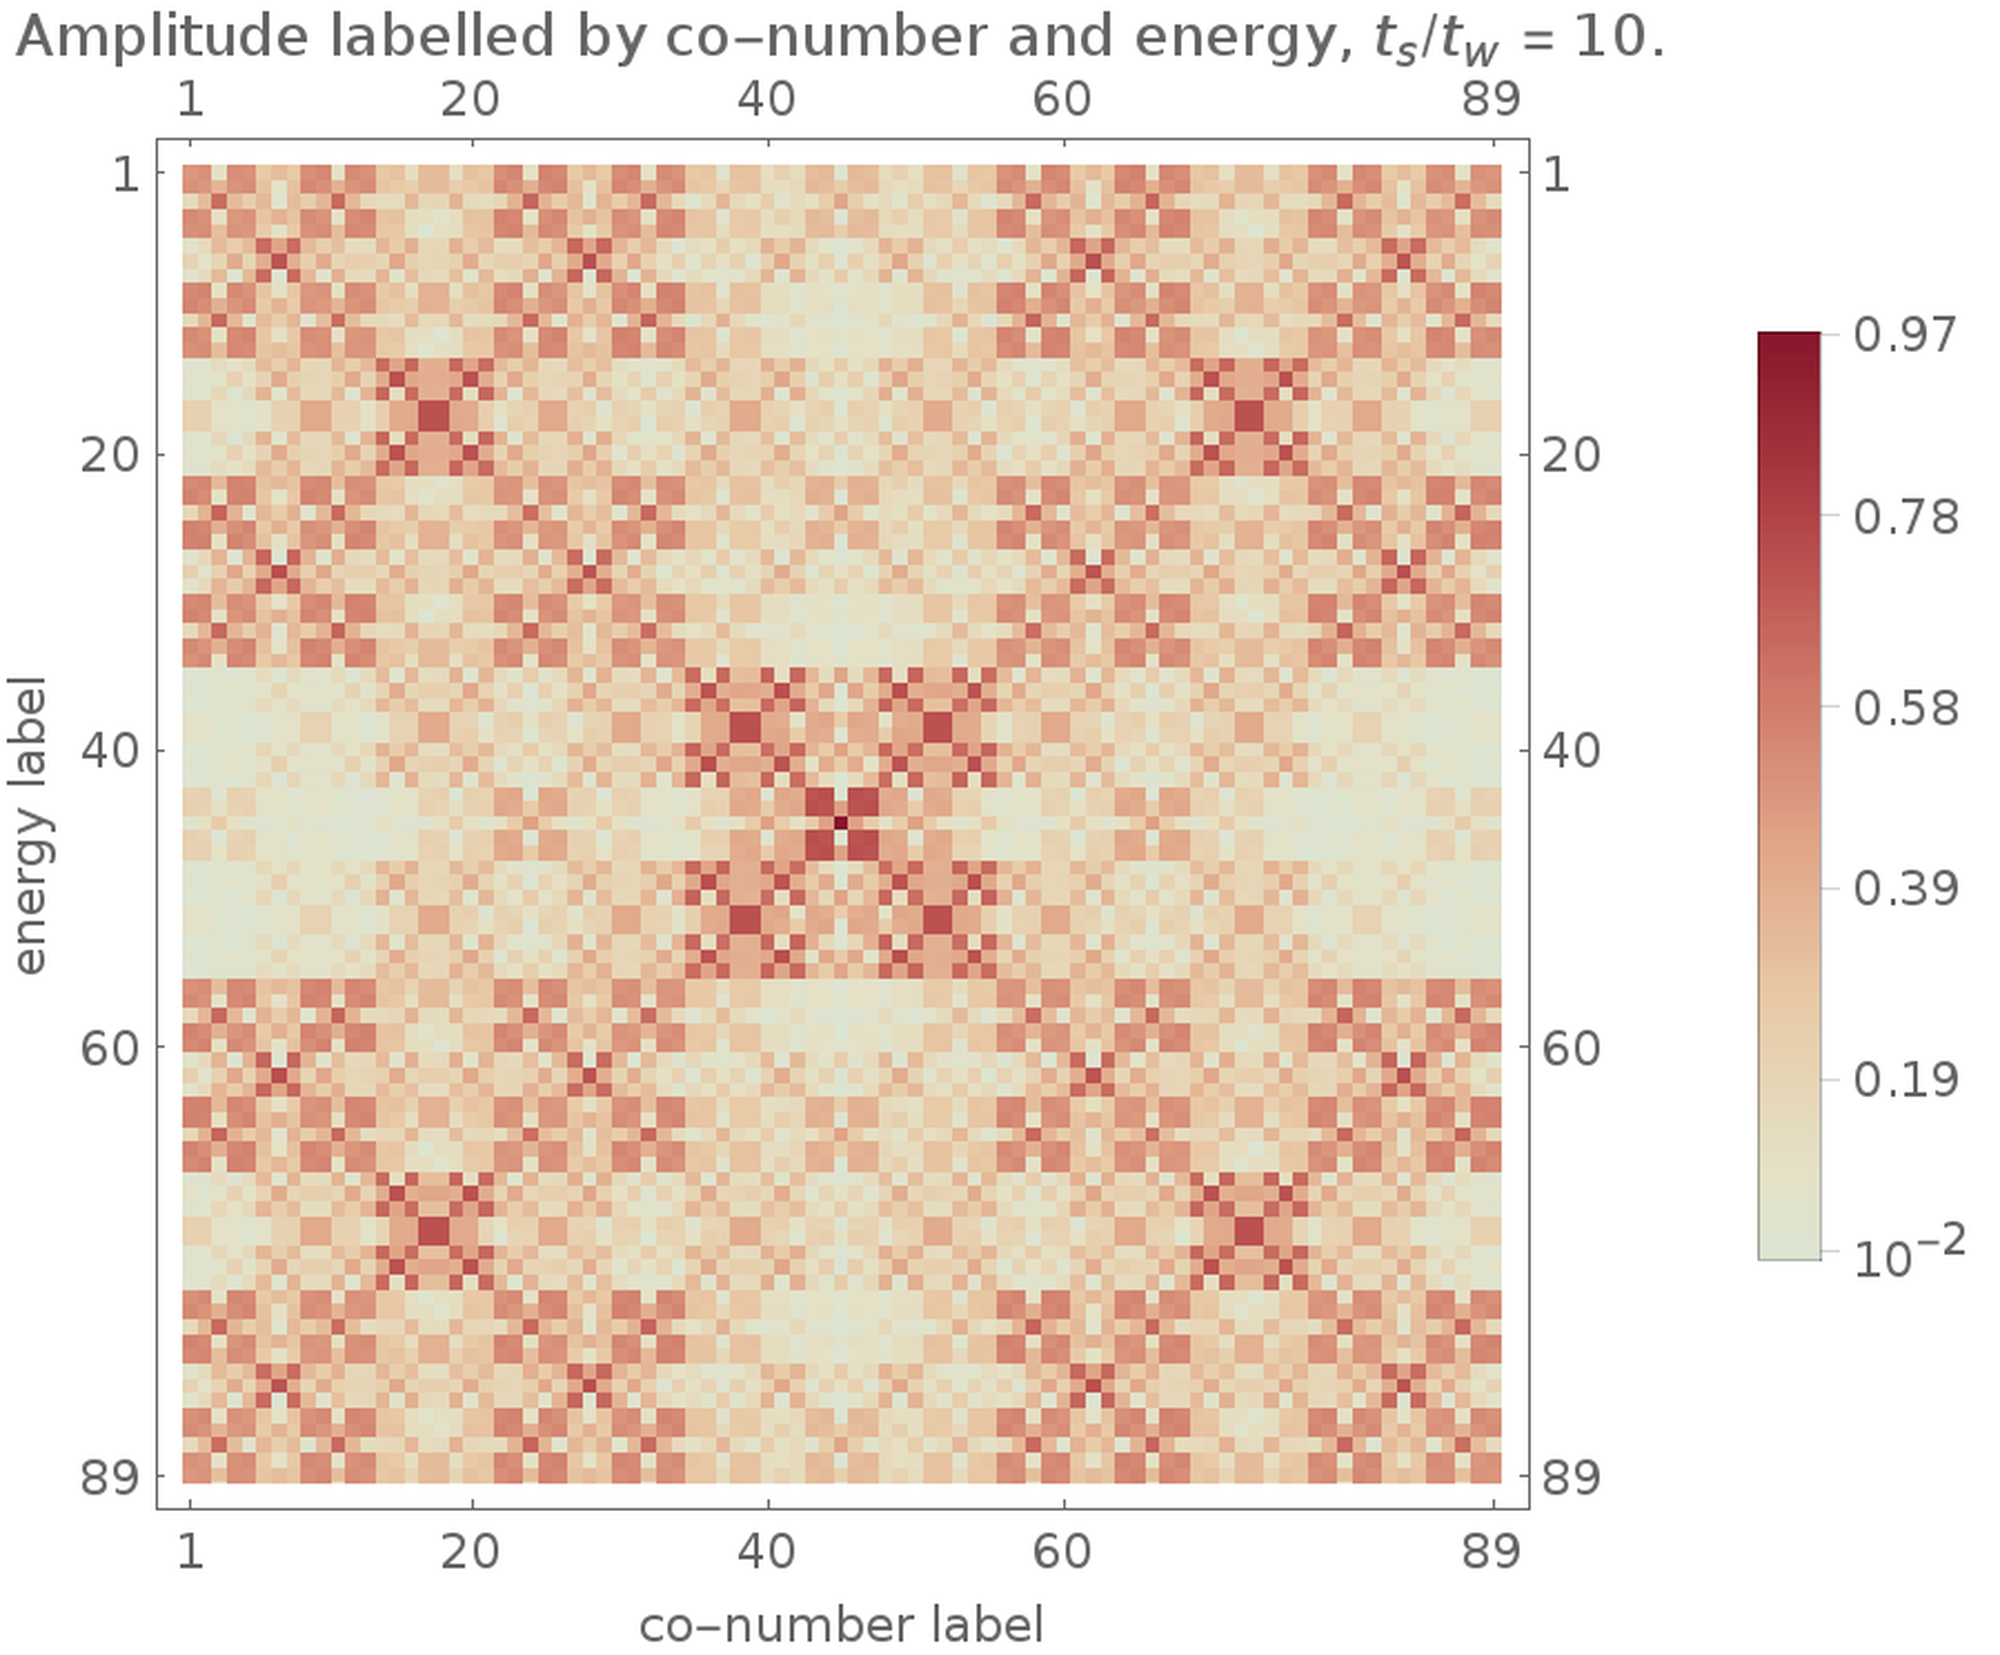
\includegraphics[width=1.\textwidth]{img/wf_idos.png}
  \caption{LDoS, numerical expression.}
  \label{fig:wf_idos_num}
\end{subfigure} \\
\caption{The local density of states, as a function of the position label (in conumbering), and of the energy label, for the eigth approximant constituted of 89 sites.}
\label{fig:wf_idos}
\end{figure}

In conclusion, we have completely characterized the eigenstates of the $n^\text{th}$ approximant, and in the course of doing so, we have proved the equivalence between renormalization paths of sites and of energy levels.
To render this equivalence more obvious and visual, we can employ the conumbering of sites.
In conumbering, the first and the last $F_{n-2}$ sites of the $n^\text{th}$ approximant are molecular (bonding or antibonding) sites, while the remaining $F_{n-3}$ middle sites are atomic. 
We can repeat this reasoning recursively: amongst the first $F_{n-2}$ sites, the first and last $F_{n-4}$ sites are molecular at step $n-2$, etc. 
Thus, in conumbering, sites are naturally ordered by their renormalization path, and the ordering is exactly the same as the one of the energy levels.
So, plotting the local density of states as a function of the energy label and the site conumber, should make obvious the equivalence between renormalization paths of sites and of energy levels.
More precisely, the local density of states should be left invariant under the exchange of the site label and the energy label axes. This is indeed what we observe, both analytically \eqref{fig:wf_idos_asym} and numerically for small values of $\rho$ \eqref{fig:wf_idos_num}.

Now that we have completely characterized the spectrum and the wavefunction to leading order in $\rho$, we can derive from that expressions for the fractal dimensions of the spectrum and of the wavefunctions.

\section{Fractal dimensions at leading order}

\subsection{Fractal dimensions of the spectrum}

We compute the fractal dimensions of the spectrum using the thermodynamical formalism \cite{Halsey1986}. We define the partition function
\begin{equation}
	\Gamma^n(q,\tau) = \sum_{a} \frac{\left( 1/F_n \right)^q}{(\Delta_a^n)^\tau}
\end{equation}
where $\Delta_a^n$ is taken to be the width of the energy band associated to the energy level labelled $a$.
One can show \cite{Halsey1986} that the generalized fractal dimensions of the spectrum $D_q$ are given by $D_q = \tau_q/(q-1)$ where $\tau_q$ is defined by
\begin{align}
	\Gamma^n(q,\tau > \tau_q) &\rightarrow +\infty \\
	\Gamma^n(a,\tau < \tau_q) &\rightarrow 0
\end{align}
In practice, a good approximation of $\tau_q$ is given by $\Gamma^{n+1}(q,\tau_q)/\Gamma^n(q,\tau_q) = 1$ for $n$ large.

At leading order, the recursion relation between energies \eqref{eq:recur_spectrum} translates into a recursion relation between partition functions. 
This makes it easy to find the fractal dimensions of the spectrum \cite{Piechon95} \emph{via} the implicit equation
\begin{equation}
	2 \omega^{2 q} z^{-(q-1)D_q}+\omega^{3 q} \zb^{-(q-1)D_q} = 1
\end{equation}
Thus, we have
\begin{equation}
	D_q = \frac{1}{1-q} \frac{\log \big[\omega^{-q} \left( \sqrt{1+\omega^{-q}} -1\right) \big]}{\log \rho} + \mathcal{O}\left( \frac{1}{(\log \rho)^2} \right)
\end{equation}
In particular, we find for the Hausdorff dimension
\begin{equation}
	D_0 = \frac{\log( \sqrt{2} -1 )}{\log \rho} + \mathcal{O}\left( \frac{1}{(\log \rho)^2} \right)
\end{equation}
in agreement with the result of Damanik \& Gorodetski \cite{DamanikGorodetski}, using trace-map-based methods.

\subsection{Fractal dimensions of the wavefunctions}

The fractal dimensions $D_q(a)$ of the wavefunction associated to the energy level $a$ are defined by
\begin{equation}
	\chi_q^n(a) = \sum_i |\psi_i^n(a)|^{2q} \simlim{n}{\infty} \left( \frac{1}{F_n} \right)^{(q-1)D_q(a)}
\end{equation}
Note that $D_2(a)$ is the inverse participation ratio.
$D_2(a) = 1$ indicates that the state $a$ is extended, while $D_2(a) = 0$ characterizes a localized state.
An intermediate value $0 < D_2(a) < 1$ is the signature of a critical state, whose multifractal properties can be probed by varying $q$.

At leading order in $\rho$ the renormalization of the eigenstates is trivial. 
On a site whose renormalization path matches the one of the energy level we consider, the amplitude at step $n$ is just the amplitude at step $n-3$ if the energy is in the atomic cluster, while the amplitude is the one at step $n-2$ divided by a factor $\sqrt{2}$ if the energy is in the molecular cluster.
The division by a factor of $\sqrt{2}$ simply comes from the fact that molecular sites are in pairs.

Therefore, we have for the fractal dimensions of the wavefunction of the energy level labelled by $a$,
\begin{equation}
	D_q(a) = x_a \frac{\log 2}{\log \omega^{-1}} + \mathcal{O}(\rho^2),
\end{equation}
where
\begin{equation}
	x_a = \lim_{n \rightarrow \infty} \frac{n_+(a)+n_-(a)}{n}
\end{equation}
with $n_\pm(a)$ the number of $+$/$-$ letters in the renormalization path of $a$.
In other words, $x_a$ is the fraction of renormalization steps in which the level $a$ was in a molecular cluster.

Since $x_a \leq 1/2$, we have $0 < D_q(a) < 1$: the wavefunctions are critical, as we expect for a quasiperiodic system.
We have $x_a = 0$ for the level that has the renormalization path $00...$, ie for the energy level $E=0$, at the center of the atomic cluster. The corresponding eigenstate has a zero fractal dimension, and is thus completely localized. As we approach the $E=0$ level, $x_a$ approaches monotonously $0$ and the wavefunctions becomes more and more localized.
$x_a$ reaches its maximal value, $1/2$, for the levels having the renormalization path $++...$ and $--...$, ie for the levels $E=E_\text{min}, E_\text{max} = \pm 1/(1+z)$ at the edges of the spectrum.
The corresponding eigenstates are the most extended. They occupy a fraction $(1/F_n)^{\frac{\log 2}{\log \omega^{-2}}}$ of the sites.

It is also interesting to note that the fractal dimensions of the wavefunction does not depend on $q$: the wavefunctions are not multifractal.
We expect multifractality to appear at the next-to-leading order in $\rho$.
To go beyond the leading order -- where the interesting physics lies! -- we have to consider overlap between atoms and molecules.

\section{Fractal dimensions at next-to-leading order and multifractality}
 
At next-to-leading order the picture of molecular and atomic eigenstates and energies remains relevant, but it is now possible to form an atomic eigenstate to have nonzero amplitude on molecular sites, and vice-versa.
A complete analysis of the situation would require pushing perturbation theory to the next order.
However, as long as we are interested in computing fractal dimensions, we only need to know the correction to the wavefunctions at the sites where they have nonzero amplitude at leading order.

It is easier to encode the corrections to leading order in a multiplicative factor:
\begin{equation}
	\psi_i(a) = \sqrt{\lambda_i(a)} \psi^{(0)}_i(a),
\end{equation}
Where $\psi^{(0)}$ is the wavefunction at leading order.

Numerically, we observe that the fluctuations are negligible relative to the mean value. More precisely, we have
\begin{equation}
	\lambda(a)^q \gg \lambda(a)^{q-k} \Delta \lambda_i(a)^k, \text{~} \forall k \in [1,q]
\end{equation}
The validity of the approximation improves as $q$ becomes larger.

However, since for example an energy $E$ of the atomic cluster at step $n$ corresponds to an energy $E/\zb$ at step $n-3$, we still hope to relate the amplitudes of the atomic eigenstate if energy $E$ on atomic sites, to the amplitude of the eigenstate of energy $E/\zb$ at step $n-3$. Specifically, we are going to assume that they are simply related by scaling factor:
 \begin{equation}
\label{eq:renorm_a}
	\psi_i^n(E) = \sqrt{\lambda} \psi^{n-3}_{d_a(i)}(E/\bar z)
\end{equation}
where $d_a(i)$ is the new numbering of the site $i$ after an atomic deflation operation.

We can easily compute this factor perturbatively (see appendix \eqref{app:renorm}). We find
\begin{equation}
	\bar \lambda(\rho) = \frac{1}{1+2\rho^2} +\mathcal{O}(\rho^4).
\end{equation}
Now, knowing the amplitude of this atomic eigenstates on neighbouring \emph{molecular} sites is easy enough. We find
\begin{equation}
	\begin{cases}
	\psi^n_{i\pm1} &= \phantom{-}0 \\
	\psi^n_{i\pm2} &= - \rho \psi^n_i \\
	\psi^n_{i\pm3} &= \phantom{-}0 \\
	\psi^n_{i\pm4} &= \phantom{-}\rho^2 \psi^n_i
	\end{cases}
\end{equation}
at leading order.

\section{Fractal dimensions in the perturbative limit}

\section{Relations between fractal dimensions and universality}

\newpage
\appendix

\section{Renormalization factors of atomic and molecular eigenstates}
\label{app:renorm}

In this appendix, we derive the expression of the renoralization factors $\lambda$ and $\bar \lambda$ of the molecular and atomic eigenstates.

\subsection{Atomic eigenstates}

Let $\ket{\psi(E)}$ be an eigenstate for an energy $E$ belonging to the atomic energy cluster, at step $n$.
At first order, $\ket{\psi(E)}$ is an eigenstate of $\zb H_{n-3}$, with the sites rearranged on the $n^\text{th}$ approximant.
Therefore, at first order $\ket{\psi(E)}$ is only nonzero on some atomic sites of the $n^\text{th}$ chain. Let $i$ label one of these sites.

The fact that $\ket{\psi(E)}$ is an eigenstate of $\zb H_{n-3}$, with the sites rearranged on the $n^\text{th}$ approximant translates into the equation
\begin{equation}
\label{eq:renorm_a_first}
	\psi_i(E) = \psi_{d_a(i)}(E/\bar z),
\end{equation}
where $d_a(i)$ is the new numbering of the site $i$ after an atomic deflation operation.

Now, at the next order, some of the intensity, that was at first order concentrated only on some atomic sites, ``leaks'' on the molecular sites neighbouring these atomic sites. 
This translates into the fact that the intensity on these atomic sites is reduced by a factor $\lb$.
So, at second order, equation \eqref{eq:renorm_a_first} becomes
\begin{equation}
\label{eq:renorm_a}
	\psi_i(E) = \sqrt{\lb} \psi_{d_a(i)}(E/\bar z).
\end{equation}
To determine $\lb$, we just have to compute how much intensity has leaked out of site $i$.

\begin{figure}[htp]

\centering
\begin{subfigure}{.5\textwidth}
  \centering
  \includestandalone[width=.82\textwidth]{img/local_environment_atoms1}
  \caption{Atomic site surrounded by strong and weak effective couplings.}
  \label{fig:atom1}
\end{subfigure}%
\begin{subfigure}{.5\textwidth}
  \centering
  \includestandalone[width=1.\textwidth]{img/local_environment_atoms2}
  \caption{Atomic site surrounded by two weak effective couplings.}
  \label{fig:atom2}
\end{subfigure} \\

\caption{The two types of local environments of an atomic site. }
\label{fig:energyconf1}
\end{figure}

The atomic site $i$ we consider can either be surrounded by one weak effective bond (fig. \eqref{fig:atom1}), or by two effective weak bonds (fig. \eqref{fig:atom2}).
In both cases, it is straighforward to compute, at leading order in $\rho$, the fraction of the amplitude at site $i$ who is transferred to neighbouring molecular sites.
Note that destructive interferences result in half the molecular sites being unaffected at leading order.

As we already said, at first order in $\rho$, the amplitude in concentrated at site $i$. We call $I$ the intensity at this site: $I=|\psi_i|^2$. 
At second order in $\rho$, the intensity $I$ has spread out at neighbouring molecular sites, and therefore the intensity at site $i$ is attenuated by a factor $\lb$. We have
\begin{equation}
	\lb I ( 1 + 2\rho^2 + \mathcal{O}(\rho^4)) = I,
\end{equation}
And thus
\begin{equation}
	\lb = \frac{1}{1+2 \rho^2} + \mathcal{O}(\rho^4).
\end{equation}

\subsection{Molecular eigenstates}

\newpage

\bibliography{fractal_dimensions_quasicrystals.bib}{}
\bibliographystyle{plain}
\end{document}